\chapter{Assured Survival}
\section{Introduction}

\begin{mdframed}[backgroundcolor=black!10]
This chapter was originally written in 1969. We had intended extensive revisions; after all, much has happened since then: the U.S. began the Sprint Anti-Ballistic Missile (ABM) System; signed and ratified the ABM treaty which restricted the U.S. and U.S.S.R. to a single system defending one strategic offensive installation; abandoned our ABM systems entirely; and, under Reagan, began the research and development program known as Strategic Defense Initiative or SDI.

When we examined the chapter, we were surprised to discover that little beyond cosmetic revision was needed.

Our original analysis missed the importance of intercepting ballistic missile boosters in the post-boost phase when orbiting defense systems can attack the primary booster vehicle before it deploys its Multiple Independently Targetable Re-entry Vehicles (MIRV). This is an additional period of vulnerability which gives defense great leverage. Otherwise, the chapter stands up very well indeed.

In the first edition of this book we argued that the US ought to abandon the strategy of Assured Destruction (since renamed Mutual Assured Destruction, or MAD) in favor of a strategy of Assured Survival. We presented that argument in a series of briefings beginning in 1968 and continuing until 1983. The analysis remains valid. [1984]
\end{mdframed}

\section{Assured Destruction}
Former Secretary of Defense McNamara based the strategic survival of the United States on a policy of Assured Destruction.\footnote{This was subsequently expanded to Mutual Assured Destruction, or MAD; what the late Herman Kahn called "a suicide pact" in his seminal work On Thermonuclear War.} This was defined as the capability to assure the destruction of some specified fraction of the population and industry of the potential enemy after the U.S. Strategic Offensive Forces (SOF) had absorbed the best possible attack the enemy could launch.

To this end, the U.S. Strategic Offensive Force (SOF) was designed to be survivable, although little was done to make it flexible. Polaris missiles and nuclear submarines were built. A force of 1,000 Minuteman missiles was deployed, although a larger force was deemed necessary by the Air Force. The Minuteman silos were hardened as best they could be, which did not make them invulnerable, and the Minuteman command structure was given redundancy. The bomber force, thought to be vulnerable to the enemy first strike, was allowed to become obsolete and decline in numbers. The bombers were not replaced by newer types until the 1980's, although systems were designed much earlier. In 1970, Congress approved research and development of a long-range supersonic bomber, the B-1, but it did not appear in inventory until the late 1980's because the program was halted during the Carter Administration. McNamara had intended, consistent with his strategic doctrine, that the strategic bomber would vanish forever from both U.S. and Soviet arsenals.\footnote{One of the most far reaching decisions made by McNamara was canceling the highly successful X Programs in the name of arms control. This action was consistent with the theory of arms control: the X projects were a continual source of new military technology. New military technology is precisely what arms controllers don’t want.}

Missiles of that era which were slow to react and believed not to be survivable were eliminated from the inventory. Overseas-based missiles were withdrawn, chiefly because of explicit or implicit executive agreements made during the Cuban incident of 1962. The capability of the U.S. high command to fight a nuclear war was regarded as far less important than the capability to achieve assured destruction of the aggressor.

McNamara began his reign by denouncing the "spasm war," the sole purpose of which was destruction of the enemy society, and said he was replacing the spasm war plan with a policy of flexible response;\footnote{The story is told that in the first days of McNamara's tenure as Secretary of Defense, he invited the Commander in Chief of the Strategic Air Command (SAC) to explain the US strategic war plan (known as the Single Integrated Operational Plan or SIOP). After the review, McNamara said in horror "General, that's not a war plan! All you have is a kind of horrible spasm."}

however, by the time he left office the entire strategic offensive force was geared to Assured Destruction and therefore to a spasm reaction. By forsaking flexible systems such as manned bombers, mobile ballistic missiles, and on-board guidance systems for ease of retargeting, the United States had technologically locked itself into a situation in which the only flexibility of the response would be "how much is left of our force, and what can we launch?"

Much of even this limited flexibility was illusory. The enemy's reserves and refire capabilities made our surviving missile force vulnerable to renewed attack unless it was launched quickly after the initial strike. Because of our lack of adequate air defenses, the enemy could destroy our unlaunched missile force with manned aircraft (even aircraft as inappropriate as refueled medium-range bombers). Without counterforce capabilities to destroy the Soviet strike forces, the United States had no choice but the spasm reaction to any enemy attempt to eliminate our strategic systems. We could not seek to reduce or destroy his ability to make war on us, because we had chosen not to construct forces capable of flexible operations. We had, almost completely, predetermined our strategy for years to come.

Thus, the United States had no alternative but Assured Destruction. If we failed to deter an enemy attack, the President would be left with only one option for retaliation: An attack on Soviet urban industrial targets. In the parlance of the time, this was known as a pure countervalue attack. We could fight no other kind of war. With our land-based systems dependent upon early launch to assure that they could be launched at all; with no flexible retargeting capability for this force; with no reconnaissance capability to allow us to know which enemy sites were empty and which were being prepared for refire; and with the Polaris force having insufficient accuracy for anything other than a countervalue strike, flexible response took on a note of irony.

\section{Soviet Strategic Doctrine}
In contrast to the United States, it would appear that the U.S.S.R. adopted a policy of Assured Survival. That is, the Soviets installed substantial defenses and counterforce weapons to limit damage from U.S. retaliation. While such counterforce capabilities are consistent with development of an "out of the blue" first strike capability, they also allow the Soviets more flexibility in responding to escalating tensions. Under some post-strike conditions the U.S. might be self-deterred from retaliating at all.

Whether they have been successful in this policy may be questionable, but the point is that they chose a reasonable strategy while our professed strategy led to deployment decisions that forced us into a posture that was the opposite of what we intended.

Presumably the Soviets have been unable to guarantee that U.S. retaliation will not bring destruction above the deterrent level. On the other hand, since the United States has conceded the initiative of striking first, the Soviets do not need to be overly concerned about the U.S. policy of Assured Destruction: the level of destruction is essentially a function of the level of success in the first strike. The lack of U.S. active defenses augmented the chances that such success might be considerable, and made it unnecessary to use any large part of the Soviet strategic budget for development of penetration systems.\footnote{This is presumably one reason for Soviet opposition to the Reagan SDI studies.}They could and did concentrate on large payload capacity, accuracy improvement, and sheer numbers of offensive weapons, hoping to exploit their numbers and large payloads more fully when multiple reentry vehicle technology was adequately developed. The rest of their budget could go to testing and development of strategic defense, to which they traditionally have allocated huge resources.

\section{Requirements of Assured Survival}
The United States has never developed an actual policy of Assured Survival. The Safeguard defensive system, abandoned after the ABM treaty, was intended to protect the SOF, not our people. Although President Reagan clearly intended the Strategic Defense Initiative as a means of protecting the American people, our strategies and doctrines are still based on a policy of Assured Destruction, and to the extent that there is bi-partisan support for SDI it is largely built around the protection of our SOF.

Defense of the strategic retaliatory force is, of course, better than no defense at all; but the moral objections to Mutual Assured Destruction are unchanged by deployment of weapons intended solely to protect missile fields.

In any event, the requirements for Mutual Assured Destruction are no less dynamic than those for Assured Survival. Deterrence through MAD is not automatic. In 1970 we pointed out at least one way that deterrence could fail through nuclear blackmail.

US strategic nuclear forces are offensive only. Suppose, then, a Soviet attack directed solely against our strategic force, with the intent of reducing the assured destruction that our damaged force, further reduced by Soviet defenses, would be able to accomplish. The result might well be that the President would question whether the surviving force would be sufficient to destroy the enemy's war-making capability.

The Soviets could then point out that the launch of our surviving force would be suicide for unprotected U.S. cities. The Soviet commanders would, of course, have held back hardened and mobile forces sufficient to destroy many American cities, using their soft-based and reloadable ICBM installations in the initial strike. Our president would be faced with a most difficult moral choice. He could either launch the SOF against Soviet industry and population centers or surrender. Doubtless, the surrender terms would be made easy to accept -- initially. Whatever happened to the United States, Europe would have no choice but surrender.

Because the United States concedes the first strike to the Soviet Union, Assured Survival is a policy more expensive for us than for the enemy. We must have an Assured Destruction capability as a part of Assured Survival; but we must also have active defenses and forces capable of defeating the enemy in nuclear aerospace battle.\footnote{It is very important to understand that the alternatives to strategic defense are grim: one must either adopt a policy of launch on early warning, or watch deterrence fail as the enemy realizes he can overcome the retaliatory force with a properly planned first strike. Launch on early warning is dangerous and destabilizing policy, and even that can be defeated with a well planned pin-down strike.} The most pressing military problem of the free world is to provide active defense against the strategic striking power of any would-be aggressor. Active defense is also the most technically difficult of the current military problems. It becomes no easier with time; the longer defense technology is held back, the more difficult the problem becomes because offensive power is growing. Yet strategic analysis indicates that a strategy of Assured Survival will be far more valuable to the free world than one of Assured Destruction.

There are two basic methods to provide Assured Survival. The first, construction of a force sufficient to destroy the enemy striking force in a preventive attack, is not feasible for an open society; if it were constructed it could not be launched by Western statesmen without severe provocation. Even a preemptive strike appears to be very difficult. The problem, it should be noted, is not symmetrical. A secretive society without scruples about aggression can achieve a decisive first strike capability far more readily than an open and peaceful government.

U.S. SOF systems are openly deployed after years of debate in Congress. Their nature, numbers, and locations can be known with considerable confidence. By contrast the U.S.S.R. can build and deploy weapons whose very existence is only speculation in the West.

Furthermore, U.S. concession of the first strike to the other side allows the Soviets to employ large missiles launched from soft pads. Thus to say the United States may be unable, given the present state of weapons technology and sociological factors, to achieve a full counterforce capability is not the same as saying that the Soviets cannot achieve it.

Note that in the above analysis we say nothing of intentions. As we write this the Gorbachev regime appears to be interested in reduction of strategic forces and the achievement of nuclear stability. We would be more convinced of this if the Soviet Union did not continue to maintain four separate missile production lines running at full capacity to produce ICBM's; but even if we assume that the current Soviet leadership sincerely desires peace and detente, it may not be desirable to bet the survival of the United States on the stability of the Gorbachev regime.

The second method of achieving Assured Survival is through active defense, coupled with sufficient counterforce capability to threaten the enemy's residual or holdback forces. Active defense also serves to prevent destruction or extensive damage to the United States by a third power. In fact, an adequate program of active defense will ensure that, whatever our capability against the U.S.S.R., the American people will not be hostage to anyone else. There are at present no other powers capable of overcoming the defenses we could construct with present technology, and by the time others achieved penetration capability the United States could easily update the system to accommodate new technology. There are other benefits to active defense. They include the "fallout" benefit of assured adn economical access to space; and control of accidental or catalytic nuclear war, which we will discuss below. Nevertheless, the primary value of defense is its contribution to a policy of Assured Survival.

\section{The Case Against Active Defense}
\begin{mdframed}[backgroundcolor=black!10]
The following analysis was written in 1970, long before the SDI debates. We see no reason to change it.
\end{mdframed}

There are two primary arguments against active defense, each in turn divided into two schools. The two broad classes of arguments against defense are theoretical and technical-economic.

The basic theoretical argument against defenses is that they might work. By so doing, they reduce the casualties that would be incurred in a nuclear war, and thus make that war more "rational" or possible. If decision makers know their national survival is assured, or believe this to be the case, the argument goes, they will be more reckless in making nuclear threats, and sooner or later the war will begin. According to this theory, the American and Soviet populations are hostage to each other, and ought to be. Through this massive exchange of hostages, we ensure peace.

The second theoretical argument against defense, often made by the same people who support the first argument above, is that the system will not work. Instead, all the defense systems will do is force each nation to construct strategic offensive forces that can penetrate the enemy defenses. This, they say, will "trigger another round in the arms race," resulting in great increases in SOF on both sides. The defenses will then be useless and vast sums of money, which should be put to work by other agencies of the government, will have been wasted. Most adherents of this view have a number of projects they believe the government should support with resources that might otherwise have gone toward a policy of Assured Survival.

The primary technical-economic arguments against defense are, first, that it cannot work, or that we simply cannot afford a system that will work. Complete defense is not possible at any price, and partial defense is prohibitively expensive. A second school contends that this argument is probably true, but that even if it were not, we would be better off using the money to construct new Strategic Offensive Forces, on the basis that the aggressor will be more easily deterred by the prospect of more complete destruction of his homeland than by the possibility that his attack will not be successful.

There are variations on those themes, including some unlikely combinations of them, but they all reduce to one or more of the basic points.

\section{Discussion}

The first and last of the above contentions reduce to the argument for deterrence as opposed to defense: Assured Destruction against Assured Survival. They are vulnerable to the same objection as is the deterrence thesis itself, namely, that an opponent with a rationality that differs from your own may not accept your logic; a stupid one may not understand your rationale; a very clever one may devise a method of neutralizing your force, either through a first strike, defense, or a combination of the two with psychological means; and a timid, frightened, or simply humanitarian president might prefer surrender to the deliberate killing of millions of nonbelligerent enemy nationals. The deterrence thesis of a balance of terror runs counter to Christian ethics and the doctrine of Just War, although, if there is nothing else to depend upon, preservation of the peace through Assured Destruction is in our judgment preferable to surrender or war, even on purely humanitarian grounds.

Furthermore, by abandoning defense on entirely theoretical grounds we fail to take advantage of inevitable breakthroughs in defense technology. It is becoming more and more conceivable, for example, that some form of ray or energy beam might be devised which could destroy all incoming warheads, whether delivered by aircraft, short-range submarine-launched missiles, spacecraft, or ICBM. This possibility, long considered remote, has become more than a theoretical possibility in the past 10 years.\footnote{There have been many scientific breakthroughs since this was written in 1969. These have led to dramatic developments in laser technology, used for detecting, tracking, and killing enemy missiles; development of tiny computers for on-board guidance of kinetic energy weapons; technology for construction of both ground and space-based mirrors for directing beamed energy; etc.} But if we do not have the radars and computers to detect and track incoming enemy missiles, perfection of laser kill mechanisms will do us little good.

We cannot stress often enough that technology has a habit of being richer than even the most imaginative planners predict. Technological breakthroughs in missile defense are inevitable, and we must be in a position to take advantage of them. It is obvious that the unilateral achievement of good defense, or offense-defense combinations, by the U.S.S.R. would hardly have a stabilizing effect on international politics. We doubt that the free world would become safer through such an event. If we want to survive, we cannot concede the initiative in active defense to the enemy. Defense technology is at the moment in the lower left-hand quadrant of the technology S-curve. We see no reason why it should not continue to a breakthrough.

\begin{mdframed}[backgroundcolor=black!10]
In March of 1983, on the advice of a council that included the authors of this book and General Daniel O. Graham, President Reagan challenged the U.S. scientific community to demonstrate and develop strategic defense technology. Within two years a number of such weapons were examined, and many found to be feasible. Some are listed in Chart 15
\end{mdframed}

\begin{mdframed}[backgroundcolor=black!10, frametitle={Potential Strategic Defense Systems}]
\textbf{Kinetic energy weapons}
    \begin{itemize}
        \item Space-based
        \item Non nuclear
        \item "Smart Rocks"
        \item Railguns
    \end{itemize}
\textbf{Terminal defense systems}
    \begin{itemize}
        \item Lasers
        \item Nuclear-powered
        \item Chemically or electrically-powered
        \item Single-shot 
        \item Continuous
    \end{itemize}
\textbf{Laser Basing systems}
    \begin{itemize}
        \item Space-based lasers
        \item Ground-based lasers with orbital mirrors
        \item Popup mirrors
    \end{itemize}
\end{mdframed}

The second argument, although theoretical in form, is in fact technological and economic, and reduces to a special case of the third argument. If a defense could be achieved that could not be countered by the offense, the argument against such defense on technical grounds vanishes. If this defense were obtainable at any reasonable price, the nation would be faced with the alternatives of continuing to live with the balance of terror or making the necessary sacrifices to end it through Assured Survival.

In the real world, of course, it is highly unlikely that a leakproof defense will ever be found. This does not mean that no defense is preferable to a partial defense. In any rational view, survival of some of the nation is preferable to complete extermination. We hope that those who fear that nuclear war will result in the extinction of all life on the planet would be the first to agree.

Moreover, partial defense systems greatly complicate the aggressor's war plan. A 25% attrition of enemy boosters would be a highly effective deterrent against any strike at all, since the enemy would have no way of knowing which of his missiles would be intercepted.

In 1970 there were legitimate questions about the technical feasibility of strategic defenses. This is no longer true in 1988. While there can and should be debate about the degree of effectiveness that can be obtained, and which mix of systems is optimum given the strategic threat, there is little scientific doubt about the ability of the U.S., using 1988 technology, to build and deploy ICBM defenses sufficient to intercept 50\% or more of the enemy's offensive strike. We may expect considerably higher intercept effectiveness with future technology. We stand at the very threshold of a rising S-curve.

The arms race argument is perhaps one of the most spectacular; it is also the most overworked. According to this view, all that defense would accomplish would be to raise the levels of strategic offensive forces in the inventories of both the United States and U.S.S.R., encumber each with defense systems that could not cope with the new offensive weapons, and waste a great deal of money all around. In addition, it is usually said that these mutual increases in SOF levels are themselves dangerous because they make nuclear war more probable.

The latter statement is most certainly not correct. As the mutual inventories of SOF increase, the destructiveness of nuclear war also increases, so that it becomes less and less rational to initiate nuclear hostilities for any but the most compelling reasons. Even the most dedicated advocates of the MAD strategy must admit that in general, the higher the force levels, the more stable what Albert Wohlstetter called "the delicate balance of terror."

In addition, even a minimum defense system will be able to cope with small, unsophisticated attacks such as might be launched by enemy officers against orders, insane local political leaders, or small nations hoping to trigger (or catalyze or provoke) a war between the superpowers.\footnote{
The "madman with a missile" scenario was first discussed by Herman Kahn. For a time after 1970 it was not taken seriously, but the rise of Khadafi and the Ayotolah Khomeni have given it a renewed attention. We now have the requirement for Northern/Southern Hemisphere deterrence. Defense against ballistic missiles will be necessary even if glasnost and perestroika are entirely successful.
}
Thus, the chances of nuclear war, initiated for whatever reason, are reduced by this new round in the arms race, even if the race works as predicted.

More important, the prediction is almost certainly wrong. It is far more likely that as each side develops defense technology, the defense systems will become more, not less, useful. Offensive systems to cope with the new defenses will become more and more expensive, so that fewer of them can be built. The price of the Technological War will increase rapidly. The first result of this price increase will be to force all minor powers out of the strategic picture. They may continue to be threats to each other, but after the first round of offense-defense deployment, the minor powers will never again be a threat to the superpowers. The Nth country problem vanishes, and in the highly unlikely event that detente is ever achieved, this achievement will be meaningful. There will be no pressures from allies to complicate the agreements made by the superpowers.

Still more important is the effect on the U.S.S.R. of a dramatic rise in the price of the Technological War. Soviet resources available for expansion and weapons are really quite limited compared to those of the United States. Even without U.S. mobilization, we are able to spend substantially more on defenses than our opponents--as indeed we must so long as the objectives of the United States and the U.S.S.R. are asymmetrical. Stabilizer powers always require larger forces than disturber powers because they have abandoned the initiative in military action; they must not also abandon the technological initiative, or else they no longer have the capability of stabilizing.

Soviet resources consumed in the Technological War of offensive against defensive strategic systems will not be available for other aspects of the Protracted Conflict. They would not be available, for example, to subsidize Soviet allies in the Middle East. They would not be available to subsidize Communists in Asia. Soviet naval strength would suffer. The threat to Europe would be eased. The consequence of a real escalation in the nuclear arms race, in which the weapons may be destined to sit unused, anyway, is to reduce Soviet resources for investment in the sphere where armed conflicts are fought. If the costs of the strategic arms race of defense and offense are really not high enough to accomplish that result, then they have been exaggerated, and the argument against defense weapons fails. If they are that high, the result will be well worth the expenditure. The cost of the war in Vietnam greatly exceeded the cost of a proper defensive system. The United States enjoys economic superiority over the U.S.S.R., and proper exploitation of this priceless advantage can result in real gains for the free world.

Indeed, given the professed intent of the Gorbachev administration to rationalize the Soviet economy, the result of a strategic defensive arms race might well be Soviet abandonment of the nuclear arms race in general. The Soviet Union, with it's economy in shambles, its minority races growing and disaffected, and the ruling Russians themselves becoming disillusioned, can hardly afford to repeat the past investments in strategic weapons. A shift to strategic defense would force them to choose between genuine economic improvements and refurbished missiles. Since they don't need the missiles, what they do will make their intent clear to the world.

\begin{mdframed}[backgroundcolor=black!10]
The above paragraph was written in 1985 for a special pre-publication of this chapter. As the Berlin Wall comes down and the winds of change sweep over Europe and Asia it is clear that the threat of SDI was as economically effective as we had predicted it would be.
\end{mdframed}

Finally, there is no good reason to suppose that if the United States fails to install defensive systems, the U.S.S.R. will not continue to increase the SOF. The evidence is to the contrary. Soviet SOF deployment has been dependent on U.S.S.R. technology and resources, not U.S. armament levels. [This remains true in 1989; Soviet missile production has not yet halted.] When the United States ceased to deploy ICBM systems for several years in the McNamara era, the Soviets redoubled their efforts to add to the SOF inventory and gain ascendancy. Since they continue to add to the SOF whether we install defenses or not, we would prefer that they be forced to divert some part of this budget to penetration aids and increased sophistication of their devices, rather than that they simply accumulate more and more missiles that could be used either to exterminate the last survivors or to launch highly sophisticated and effective attacks against our SOF. With very large numbers in inventory, a Soviet pin-down attack becomes far more than a theoretical possibility.

\begin{mdframed}[backgroundcolor=black!10]
In fact, since we wrote the above paragraph in 1970, the Soviet Union did precisely as we predicted. They greatly increased their Strategic Offensive Forces, then invested in SS-20's to threaten Europe.
\end{mdframed}

In our judgment, the arguments against strategic defense are basically those used against any attempt to win the Technological War. They stem from an incorrect view of Soviet motives, or an incorrect appreciation of the decisiveness of the technological theater of combat, or an incorrect understanding of the S-curve of technology. They stem from wishful thinking about the advantages of using the money that would be spent on the Technological War to eradicate poverty, or crime, or disease, or whatever other cause is favored at the time. We share the reluctance to spend money on unnecessary weapons. We have no desire to waste the resources of the American people on defense and weapons simply for their own sake. However, we recognize the grim reality of the times. The silent and decisive Technological War will be won or lost by weapons, not wishful thinking; and in time of war, especially in the early nuclear age, a nation must choose survival as the primary goal.

\section{The Case for a New Strategy}
The benefits of a strategy of Assured Survival are presented in outline form on Chart 15. Most of these have already been discussed elsewhere, and demonstrate how strategic analysis should influence technological decisions.

By protecting national leadership against nuclear attack, a defensive capability gives political leaders time to assess the nature and purpose of the enemy action and decide on appropriate responses. Without this assurance of survival of the highest authorities, the United States has no choice but to delegate launch authority to the surviving commanders or launch on warning of attack. Because survival of a general staff cannot be assured, the attack must follow a preplanned pattern, which means in effect that it must be directed against targets chosen well in advance of the conflict. This makes conduct of the war dependent on our intelligence capabilities.

We do not argue against such preprogramming, and in fact recommend it; but we would prefer to have the option of a careful post-attack assessment, and a rational response to enemy action. This can only be gained if an authority with the means of countermanding and modifying the preplanned strike can survive; and the only way to assure such survival is through active defenses.

\begin{mdframed}[backgroundcolor=black!10, frametitle={CHART 16: The Benefits of Assured Survival}]
    \begin{itemize}
        \item Ensure Survival of National Leadership
        \item Allow political control of the war
        \item Increase time for decision on retaliation
        \item Increase effectiveness and Flexibility of U.S.Second Strike
        \item Increase cost and complexity of enemy first strike.
        \item Increase credibility of U.S. guarantees to allies.
        \item Decrease likelihood of thermonuclear holocaust
        \item Retaliation need not be launched on warning.
        \item Intercept and negate small attack.
        \item Control accidental war.
        \item Control catalytic war.
        \item Advance defense technology to breakthrough; brings defense and offense to better balance.
        \item Minimize civilian losses.
        \item Environment and natural resources.
        \item Prevent genocidal strategies.
    \end{itemize}
\end{mdframed}

Active defenses will preserve more flexible means for carrying out a counter attack. By protecting our strategic offensive forces, we will have more of them, and have more options. This surviving war-fighting capability may be sufficient to disarm the enemy, thus avoiding the necessity for mutual extermination.

Active defenses may prevent the first strike from coming at all. If a technological breakthrough allows the enemy a capability of destroying our undefended missile force, it does not follow that this new technology will also be sufficient to allow him to overcome those weapons if they are defended. There has been considerable discussion of electromagnetic pulse (EMP) resulting from nuclear explosions in space. Without discussion of the technical merits of the arguments, it is obvious that if there were such an exotic kill mechanism that could disable our missiles in their silos, the carrier of the weapon with this mechanism still would have to be delivered on target. A defense capability would keep the carrier at a distance, require a much heavier attack, and disrupt the aggressor's attack pattern.

When the enemy must counter active as well as passive defenses such as hardening and dispersal, he must devote major resources to the effort. This diversion is beneficial, provided only that we have not wasted resources we might have used against him. But since the United States holds a defensive grand strategy and is a stabilizer rather than a disturber power, active defense is very much in keeping with our overall strategic posture; at the same time it requires the enemy to devote resources that might have been used to destroy us to the penetration or destruction of our defense network. At any given time, resources have a constant magnitude and are not expendable at will.

Another dramatic effect of Assured Survival is on our allies. The United States may be willing to place the U.S. at risk to prevent the takeover of France or Germany, but it would be more comforting to allies to know that, if we had to launch a counterattack against the U.S.S.R., we did so with strong expectations of survival. It would make it a lot easier for allies to believe we would in fact launch the strike. More important, it would be a lot easier for the Soviets to believe it.

Finally, by making possible a counterforce type of war, with interception of small or uncoordinated attacks against us before they destroyed much of the nation, Assured Survival through active defense would make less likely the thermonuclear holocaust that paralyzes so many of our intellectuals with fear. Accidental and catalytic war as well as war caused by third parties would no longer be total. National authority would be able to assess the effects of the enemy attack, which, if the defenses were effective at all, would have caused no great harm to our cities. It would be possible to determine whether a flight of missiles directed at us were the first wave of an attack, a pin-down maneuver intended to create a local environment through which we could not launch our missile force, or an unauthorized act. We could tailor our response accordingly.

In addition to active defense, we also require counterforce weapons. Assured Survival cannot be entrusted entirely to defense, because deterrence cannot be achieved except through offensive threats. So far as it goes, the idea is valid that the enemy will be deterred if we have an assured capability of inflicting enormous damage on his society. But if our strategic objective is to ensure that we do not suffer mass destruction, and will not have to kill millions of his noncombatants, we must be able to fight a war through to a successful conclusion. Pure defense is obviously no strategy at all; we need counterforce weapons as well.

The Soviets have grasped this essential point and unlike us have been deploying new systems; since the 1970's they have developed, made operational, and deployed 5 new ICBM's, some with nuclear payloads of up to 25 megatons as a single warhead, others equipped with multiple reentry vehicles to strike many targets with the same missile. Many of these systems have a reload/refire capability. Others can he held as a strategic reserve to use against our cities. We must have a capability of destroying that reserve force before it can be launched against us.

In summary, given acceptance of a strategy of assured survival, we must consider active defense and strategic counterforce weapons as the means for achieving that posture.

\section{The Technology of Active Defense}
The following brief and admittedly incomplete discussion of the technology of active defense is presented to put the problem in focus and to illustrate the nature of technological warfare. Active defense is one of the most complex and difficult problems posed to the planners of the Technological War. For precisely this reason, it could be one of the most decisive engagements in that silent and apparently peaceful war.

\section{The Nature of the Threat}
We can define the defensive problem more concretely by examining the many kinds of weapons that could be used against the free world. The list of weapons is formidable.

The threat of air power is still poised against the free world. This includes tactical fighters and bombers; long-range subsonic bombers; and supersonic bombers. These aircraft carry a variety of nuclear and nonnuclear gravity munitions and guided air-to-ground missiles. The Soviet air force is a formidable threat, only minutes away from NATO countries and Alaska, but still hours away from the continental United States.

Surface-based missiles have considerable variations in range. The Soviets began their program with the development of short-range and medium-range land-based and submarine-based missiles. The total force could carry a considerable weight of attack against Europe and Asia. The submarines also pose a direct threat against the Continental United States. One scenario, the so-called decapitation attack, has the war begin with sub-launched missiles aimed at Washington and other national command centers. These would arrive with a maximum of 12 minutes of warning, and, given uncertainties in detection and decision making by our warning system operators, probably considerably less effective time.

The intercontinental ballistic missiles pose the most direct and formidable threat against the United States. They can reach any part of the country. They carry large nuclear warheads. Furthermore, the ICBMs in existence today are accurate fourth-generation systems, with more capability to come. In 1964 the best estimates of Soviet capabilities predicted they would achieve 600 foot accuracies at intercontinental ranges by 1975. Technology has advanced considerably since that time. It is safe to assume accuracies of no more than 300 feet.

Global ranges have been achieved with FOBS (Fractional Orbit Bombardment Systems) and conceivably could be augmented by fully orbital systems, including those with highly eccentric and very high orbits. The Soviet missiles carry large payloads, and can accommodate decoys, multiple warheads, maneuvering warheads, and target seekers.

The missiles have paved the way for threats from space. Although this is forbidden by treaty, bombs of great size can be put into orbit. Khrushchev claimed these could be 100-megaton area weapons. Numbers of them could be orbited simultaneously so that at least one would be over the United States or Western Europe at all times. Warning of attack would be measured in minutes. There is some speculation that offensive systems will not be limited to nuclear weapons. New laboratory devices could result in exotic weapons, such as energy beams, that could be used for operations in orbit. While such concepts are years away from reality, it is important to realize that the state of offensive power is dynamic and that defensive power can and must be even more dynamic.

Hence, the aggressor has extreme flexibility in tactics. He could use a mass launch of his many systems, varying the time of impact of his weapons. He could use varying times of launch and strive for near-simultaneous impact. He could attack in waves, depending on which targets he thinks he must eliminate to attain overall success. For example, he could attack warning, reconnaissance, and defense systems on the assumption that he would sacrifice giving warning in order to ensure penetration of defenses. He could use feints and threats on the assumption that he could wear down our alert force and thus facilitate his later strike; or he could try to maximize surprise in all its forms.

\section{Defense Problems}
The extreme complexity of possible attacks greatly complicates the defense effort. It is therefore not surprising that many theorists have thrown up their hands in despair, and turned to a doctrine of offensive a outrance as the sole possible answer. They contend that against these highly sophisticated and complex attack mixtures the only tactic is one of deterrence through a threat of a counterattack directed, not at the enemy's weapons, but at his value system.

The defense picture is easier to comprehend if we break it into parts and examine each of them. Additional analytic divisions are possible, but for our illustrative purposes we divide the problem into the following categories:
\begin{itemize}
    \item ICBMs and Space
    \item Sea-launched Systems
    \item Aircraft
\end{itemize}

The first category, ICBMs and Space, is the most complex. Underseas warfare technology also is difficult, with few promising approaches, but for the submarine to deliver its weapons, either ballistic missiles or air-breathing cruise missiles, it must launch them through the aerospace. If these can be intercepted, the threat of the submarine is largely negated. The development of space based synthetic aperture radar has heralded a new breakthrough in capabilities to detect submerged missile subs.

In any event, we will examine the ICBM defense problem. We will not discuss undersea warfare and air defense, not because they are uninteresting but for the sake of brevity.

\section{The ABM Problem}
The Nature of the Attack. ICBM weapons go through four reasonably distinct phases on their way to target. They are the Boost Phase, Post-Boost Phase, Midcourse, and Re-entry (or Terminal) as shown in Figure 2. Each phase has certain characteristics.

\begin{figure}
    \centering
    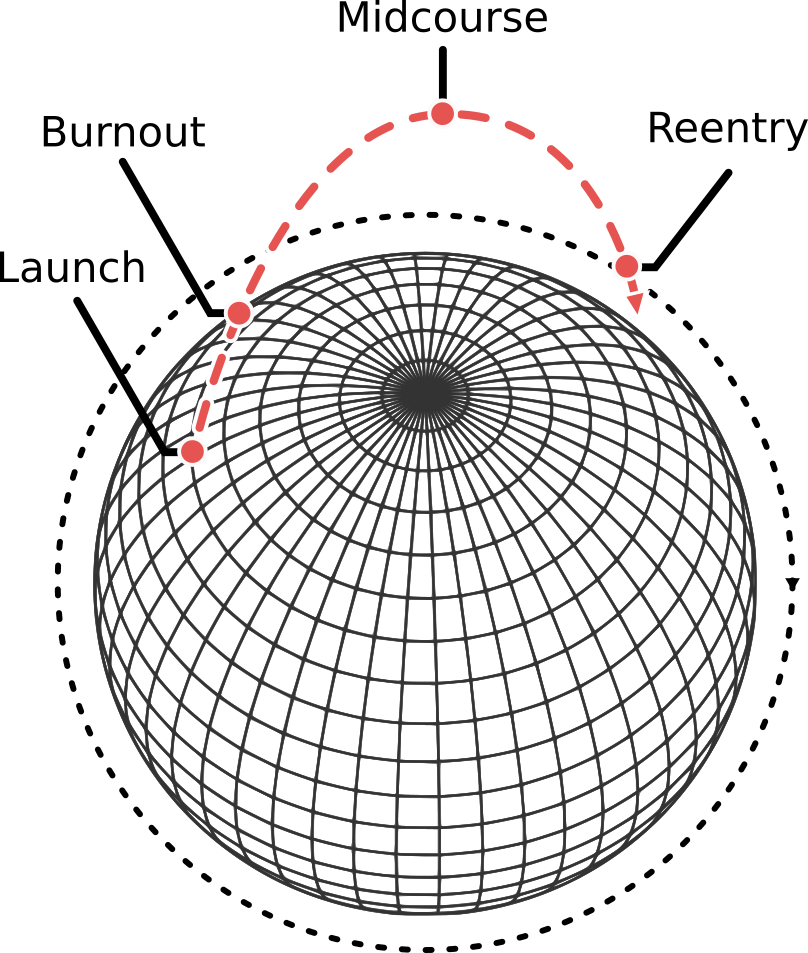
\includegraphics[width=\textwidth,height=\textheight,keepaspectratio]{./fig-2.png}
    \caption{Figure 2: Phases of ICBM Flight}
    \label{fig:icbm-traj}
\end{figure}

\section{Boost Phase}
The boost phase lasts from the time of launch until the rocket engines are shut down (burnout). The phase is characterized by relatively slow flight, necessity for exact guidance, infra-red and perhaps other radiation, and high vulnerability. Given an interceptor vehicle with the proper homing equipment in the vicinity of the missile, boost phase interception is theoretically the simplest method of active defense.

\section{Post-Boost}
After the Boost Phase, the Post Boost Vehicle, or Bus, continues on a ballistic trajectory until it reaches the point in space at which it deploys its MIRV (Multiple Independent Reentry Vehicles) and/or decoys. For single-warhead ICBM's without decoys this phase is not distinguished from Mid-course.

\section{Midcourse}
The midcourse phase lasts from burnout to reentry of the warhead into the atmosphere. A purely ballistic missile during this phase is passive; it is cold, gives off no radiation, and most of the time moves at tremendous speed. It could reach a height of 700 miles or more. Some ICBM systems are designed to make use of midcourse correction, a maneuver in which the course of the missile is determined, its impact point predicted, and some kind of power applied to the vehicle to move the impact point closer to the target. If midcourse corrections are applied, the missile must radiate, and will be easier to detect and track.

Multiple independently targeted re-entry vehicles will also radiate during some part of midcourse flight, as the warheads are deployed from the bus.

Geography dictates that the midcourse phase for missiles directed at the United States from the USSR must pass over large uninhabited areas such as the Arctic icecap, or Antarctica. This is a theoretically desirable location for interception, as damage caused either by the interceptor warhead or by premature detonation of the missile warhead will be negligible. At the same time, interception in this region of flight is more difficult, as decoys of small weight cannot be distinguished from the bomb-carrying reentry vehicle or vehicles.

\section{Reentry or Terminal Phase}
In the days of the Safeguard system the Re-entry, Terminal, or "end game" phase, in which the incoming warhead must pass through some or all of the atmosphere before it reaches its target, received a great deal of attention. By reentry time, the reentry vehicle (RV) has long since separated from its powered booster and is flying a more or less predictable path, although the shape of the RV, plus sophisticated techniques for moving its center of gravity, allow limited maneuvering capability for evasion of defenses or accurate target-seeking.

The RV leaves a detectable ionized wake in the atmosphere. It is small but vulnerable, particularly in its initial stages where limited distortion of its shape or damage to its heat shield will destroy it completely. This phase takes place over the United States, and thus requires that the interceptor vehicle use a non-nuclear weapon, or a very clean warhead of limited yield to avoid damage to the population below

\section{Interception Possibilities}
Boost Phase and Pin-down. The most intriguing intercept possibility is some form of destruction during the boost phase of the enemy missile. This was once studied as Project BAMBI (Boost Anti-Missile Ballistic Interception), but the results (1959) were discouraging. Since that time, more promising approaches have been developed, but unfortunately they are more available to the enemy than to the United States.

The tactic that appears to have the largest prospect of success is a pin-down attack. In this attack, warheads fired from the defender's homeland or from space are detonated in the atmosphere over enemy missile bases. As the boost phase of an ICBM lasts several minutes, and the missile is quite vulnerable during that time because its guidance system is active and it is undergoing acceleration, any nuclear detonation nearby will render it useless if it takes place during the first few minutes of launching. The missile is no longer in its protected silo, and it is moving slowly through the atmosphere. Blast can push it off course; electromagnetic pulse can negate its guidance commands; hard radiation can destroy its guidance computer; or heat can even detonate its unburned fuel. A multimegaton warhead detonated within several miles of an ICBM in boost phase can destroy the missile.

To employ a pin-down tactic, then, it is necessary that a string of nuclear warheads be timed to arrive and explode at two to five minute intervals over each missile farm. This pin-down attack continues until other weapons arrive to destroy the missiles in their silos; none will rise through the pin-down detonations. Successful pin-down attacks require many warheads, but not an excessive number; for example, the entire Minuteman force of the United States might be pinned down with about 100 warheads per hour. Given multiple warheads, this could require as few as 20 enemy missiles per hour, surely not an impossible number.

The advantage of this technique goes mostly to the surprise attacker, who may begin his strike with a much smaller level of effort. He does not have to destroy the entire enemy missile force in his first attack wave; he merely pins them down until other weapons, including both ICBM's and manned bombers, arrive to finish the job. Only a few warheads are seen by the defender's early-warning system if pin-down tactics are employed; by the time the victim realizes what has happened, it is too late to launch his missile force.

Pindown attacks can be launched in a variety of ways. The most plausible strategy calls for the initial strikes to come from submarine-launched missiles, followed by ICBM's. However, if the original pin-down detonations come not from ICBM but from apparently peaceful satellites, there may be no warning at all before the force is trapped. Unless the defender has space weapons and manned bombers already in flight, he will not be able to employ pin-down tactics of his own because his force cannot get through. He has been denied access to space.

An alternate technique for boost-phase interception requires that space interceptors be constantly over the enemy territory. Keeping a sufficient number of interceptors continuously ready for action and over the enemy territory is costly, although not impossible. Advances in technology -- lasers, neutral particle beams, non-nuclear "smart" weapons -- make it possible to attack missiles as they rise. This will be discussed in more detail in the update sections below.

On the other hand, a smaller number of space-based interceptors employing pin-down tactics can be highly useful. Moreover, even a few boost-phase interceptors with large yield weapons in random orbits severely complicates the enemy's first-strike planning. He must plan to make this launch when there is no interceptor over his country (assuming that he knows what is and what is not an interceptor.) If he sends his attack out in waves, a single explosion in their midst can destroy a very large part of his force. The satellite-based, boost-phase interceptor can be useful to the attacker and it is also a possibly valuable component of the defensive arsenal. It can be coupled with manned, defended satellites that control the interceptors.\footnote{
Such satellites are, of course, vulnerable to attack. However, their destruction would provide unambiguous warning of immanent attack.} Manned space components can be useful in any phase of interception.

[By 1980 it was clear that space-based components of a defense system could accomplish boost-phase interceptions using laser kill mechanisms (space battle stations) or through kinetic kill ("smart rocks" or "brilliant pebbles"). The American Physical Society and IBM Fellow Richard Garwin chose to ‘analyze’ this possibility by ignoring the space-based elements, and acting as if the interceptor had to be launched from the continental United States. They then claimed that the proponents of SDI were so stupid as to believe that the intercept mechanisms could exceed the speed of light. When it was pointed out that they analyzed a system no one had ever proposed, they continued with their derisive reports. Fortunately they were ignored by the President although not by most of the intellectual establishment of the United States.]

Post-Boost Phase. The missile in Post-Boost phase is vulnerable to attack from orbiting weapons, whether directed energy or non-nuclear, because in order to deploy decoys or MIRV it must perform thrusting operations, and thus will be visible to space-based sensors.

Midcourse. Theoretically, midcourse interceptors would best be based in the geographical area in which interception is to take place. That is, they should be based in the Arctic, probably on mobile platforms that could be either airborne or seaborne. Radars and other components of midcourse interception can be based in space or on land or at sea.

The midcourse interception problem is complicated by the fact that detection of the ICBM is hardest in this phase of flight. Its altitude is very great, and it is or can be cold and nonradiating. It may be accompanied by decoys, and it leaves no wake. However, the problem of intercepting large clouds of incoming warheads is not insuperable. Our ability to intercept this type of attack would complicate the attacker's war plan: not only must he invest in decoys at the expense of warheads, but he cannot be certain how much of his attacking force will get through. The fact that midcourse interception can be made difficult or impossible does not mean that it has been made so. Whether this kind of intercept capability is a prudent investment for the free world is a technical and economic question; but it should be noted that a relatively small capability will still greatly complicate the attacker's planning problems and decrease his confidence.

If we remember that the purpose of defense capability is Assured Survival, and that this is best achieved if the attack never comes off at all, the midcourse interception problem assumes more manageable dimensions. We are not greatly interested in a capability for midcourse interception of a few small warheads or decoys. These can be destroyed by area and point defenses based in the United States, near the potential targets. What is desired is a capability for complicating the attacker's battle plan, and for diminishing or destroying clouds of salvoed weapons launched at us. Thus, not only can anti-missiles with relatively large but standard or improved warheads be employed but also the tactic of "threat-tube sterilization" is applicable.

This technique is based on the fact that an ICBM leaving a known location for a known destination can fly only one path, predictable in advance. It must travel through a "threat tube" in space. Properly designed weapons that vector their effects along a single direction rather than in a spherical burst can be used to destroy everything in the threat tube.\footnote{One approach to vectored energy weapons is to employ debris, steel slugs, or other physical objects -- a sort of atomic grapeshot. Another is to focus radiant energy.}The presence of decoys becomes irrelevant. Such directional weapons are highly expensive (because they must be boosted into space), and would hardly be employed against single warheads, but as a system to be used against a heavy attack they show promise.\footnote{As access to space becomes cheaper, such weapons become more feasible. Ultimately such defenses would be in orbit.}

Midcourse interception becomes a matter of area defense in the latter portions of ICBM flight. A long-range, interceptor designed to defend against enemy RVs over a wide range and area can be used in midcourse interception as well as in the terminal phase or end-game. It can also be used to deliver threat-tube sterilization devices. Thus, although the best theoretical midcourse interceptors should be based in the geographical area of intercept (to cut down time of flight before intercept, allow larger payloads, etc.), it is not absolutely necessary that they be based there. Area defenses in Alaska and Greenland would, or course, be useful for both missions.

If it is technically feasible, an area defense system using airborne or sea-based platforms with sensors and weapons would be valuable. Problems of location, guidance, communications, and payload complicate the matter, but the mobility of such systems would allow them to be used in defense of allies. A capability for forward deployment to provide allies with not only deterrent protection but active defense would be of immense value.

Space-based defense systems, which might make use of vectored effect weapons or, in years to come, energy beams, including laser weapons, could also be useful in defense of allies.

\begin{mdframed}[backgroundcolor=black!10]
The feasibility and important of space based defense systems has dramatically changed since the above was written in 1969. The SDI program has identified a number of ways that such systems can be employed. In 1969 we advocated designing space exploration programs to determine the feasibility of space-based defensive systems; now, in 1989, it is clear that they are vital for a strategy of Assured Survival.
\end{mdframed}

Reentry. Terminal interception of the incoming RV after it has entered the atmosphere is the most-discussed type of ABM system, and has been adequately summarized in many publications. We confine the discussion below to a few observations.

End-game or atmospheric interception can be roughly divided into two types: area and point. Area defenses employ relatively long-range interceptors which can be used over a broad geographical area. Because of their time of flight, they must make interception at relatively high altitudes.

Point defenses, in contrast, can defend only specific targets. The point-defense concept, however, has two advantages. It may make use of somewhat smaller interceptors (although the tremendous accelerations required because of their short time of flight make their design and construction very complex); and, because interception takes place at lower altitudes, low-weight decoys have been stripped away from the warhead by the atmosphere and target identification is more or less assured. It is not worthwhile for the enemy to employ high-weight decoys, because the cost of their delivery is sufficiently high that it would be preferable simply to add another warhead.

\begin{mdframed}[backgroundcolor=black!10]
Although the U.S. abandoned the SPRINT and other point defense missiles developed in the late 60's, a number of new point defense systems were developed in the 1970-1988 period. These include high velocity/high fire volume guns. There is little doubt of the feasibility of point defense of hard targets such as missile silos. We do not know of adequate point defenses for soft targets such as cities, which must be defended by weapons that intercept at longer ranges.
\end{mdframed}

Discussion. This general and non-technical description of some of the problems of active ICBM defense is intended to serve as a background for the recommendations we make below. Our purpose is to show strategic considerations, and how they affect technological decisions and the management of the Technological War.

The offense-defense duel is summarized on Chart 16.

\definecolor{Silver}{rgb}{0.752,0.752,0.752}
\begin{table}
\centering
\caption{CHART 9: Strategic Analysis}
\begin{tblr}{
  row{1} = {Silver,c},
  row{2} = {Silver},
  cell{1}{1} = {c=5}{},
  cell{3}{1} = {Silver},
  cell{4}{1} = {Silver},
  cell{5}{1} = {Silver},
  cell{6}{1} = {Silver},
  cell{7}{1} = {Silver},
  cell{8}{1} = {Silver},
  cell{9}{1} = {Silver},
  hlines,
  vlines,
}
\textbf{CHART 16: Interception Concept}      &                      &                                                          &                                                                                                    &                                                         \\
{\textbf{Technical}\\\textbf{Problem}}       & \textbf{Pin-down}    & \textbf{Boost Phase}                                     & \textbf{Midcourse}                                                                                 & \textbf{Reentry}                                        \\
\textbf{Detection}                           & --                   & Simple                                                   & Very Difficult                                                                                     & Feasible                                                \\
\textbf{Acquistion}                          & --                   & Simple                                                   & Difficult                                                                                          & Feasible                                                \\
\textbf{Tracking}                            & --                   & Simple                                                   & Very Difficult                                                                                     & {Feasible\\Fast action\\required}                       \\
{\textbf{Decoy}\\\textbf{Discrimination}}    & --                   & {Problem\\nonexistent}                                   & {Very Difficult\\to impossible}                                                                    & {Feasible to\\Simple}                                   \\
{\textbf{Interceptor}\\\textbf{Launch}}      & {Routine\\ICBM}      & {Highly difficult\\interceptor\\must be in\\target area} & Routine                                                                                            & {Very fast response\\required; feasible\\but difficult} \\
{\textbf{Timing \&;}\\\textbf{Guidance}}     & Routine              & {Routine;\\present state\\of art}                        & Feasible                                                                                           & {Feasible but\\difficult}                               \\
{\textbf{Vulnerability}\\\textbf{of Target}} & {Highly\\vulnerable} & {Highly\\vulnerable}                                     & {Less vulnerable\\Large yeild\\weapon\\employable\\Directed effect\\for sterilization\\employable} & {Atmopsphere\\attenuates\\weapon effect}                
\end{tblr}
\end{table}

\section{Passive Defense}
All active defense programs must be coupled with passive defense or shelters. The usual objections to shelters are expense and their so-called provocative nature. Although limitations of space prevent detailed analysis of these arguments, we will briefly discuss each.

To deal with the second objection first, shelters are no more provocative than any other defense measures, and less so than offensive weapons. Providing a capability for protecting the U.S. civilian population can provoke only those who intend to kill American citizens. We have not found the well-known Soviet civil defense programs provocative.\footnote{
As of 1988, the Soviet Union continues to require every citizen to undertake some thirty hours of instruction in civil defense, and maintains a system of fallout shelters. It is said that the Soviet population doesn't take this training seriously.}
 
With regard to cost, no one imagines that even partial shelters will be cheap; yet, with minor modifications or new construction, many shelter spaces can be created at very low cost. Urban renewal and Interstate highway construction offer excellent opportunities. Bridge abutments, overpasses, etc., provide heavy concrete and earth-filled structures that could be made with hollow spaces to provide shelter. Basements of new office buildings supported by public money can also be used. Shelters are costly if they are constructed as shelters; but if they are included in new construction the additional costs are small.

\begin{mdframed}[backgroundcolor=black!10]
Since this was written, the Interstate Highway System, which was originally intended to incorporate shelter spaces in the overpasses and bridge abutments, has been completed without making any contribution to civil defense. We can only hope that those who chose to strip the nation of the means for assuring the survival of at least part of the population were correct.
\end{mdframed}

Assured Survival will not require a massive expenditure for shelters. It will require intelligent analysis of existing structures and future construction to provide passive defense to protect the population. Combined with active defense, intelligent shelter identification and construction can greatly reduce the possibility of "assured destruction" of the United States.

\section{Laser Weapon Systems}

\begin{mdframed}[backgroundcolor=black!10]
We have left much of this section as written in 1969. This is not merely braggadocio to show off the correctness of our predictions. The point is that those predictions were a result of the principles developed in this book. If laser technology had not proven to be the right path, something else would have; but in 1969 lasers and beam technologies in general appeared to be a good bet because of their momentum, and because if they did pay off, they would pay off big.
\end{mdframed}

There are many indications that laser technology is on the threshold of a major breakthrough. The laser offers such outstanding potential advantages for missile defenses that it cannot be ignored; it may be the defensive answer to the preponderance of offensive power generated by the ICBM. Lasers already seem to be the proper defense of ships against missiles such as the Soviet-constructed Styx with which the Egyptians sank the Israeli destroyer Elat. Some strategists even foresee the end of the ICBM as a modern weapon. They say the laser has sufficient potential to eliminate the ICBM threat and usher in a new era when defense has the preponderant advantage, rather than offense. This may be far-fetched, but it is something to think about.

\begin{mdframed}[backgroundcolor=black!10]
We have left the above as it was originally written in 1969. Now, in 1988, it is clear that several varieties of lasers have great potential for defense against the ICBM.
\end{mdframed}

The laser is a kind of energy beam; it projects a tightly-focused beam of high-energy coherent photons with power sufficient to melt holes in aircraft, missile booster, and possibly reentry vehicles. The range at which it can do this is at present (1969) rather short; but this is a function of the focusing of the beam, and research now indicates that it may be possible to extend this range to enormous distances. Specialized short-range Army lasers have already punched fist-sized holes in armor plate at ranges of several hundred yards.

The primary advantage of the laser for missile defense is that it acts almost instantaneously; the killing power travels at the speed of light, 186,000 miles per second, and consequently the capability to locate an incoming RV is sufficient to aim the weapon; the enemy vehicle need not be tracked for long distances. As the laser is a multi-shot weapon, decoy discrimination becomes less important; there is time to shoot down many incoming objects. Unlike an atomic ABM warhead, the laser kill mechanism does not contaminate the detection environment; the laser leaves no ionized cloud behind to blind its own radars.

Thus, laser defense systems offer enormous potential. Tracking enemy reentry vehicles is simplified; multiple installations become possible; there is little chance of running out of ammunition, as is possible when defenders must use interceptor vehicles. Shipboard installations become a distinct possibility, thus giving mobility to the defense and making a surprise attack on defensive installations much more difficult.

The present state of laser technology is, of course, highly classified. However, it is obvious that many of the early technological difficulties such as low efficiency and impossible power requirements have been overcome. We can expect continued advances in this field, and the Department of Defense is investing in laser technology. A Congressional appropriation committee member has questioned the value of research into "something that is away in the distance, 5 or 6 or 10 years," demonstrating again the problem of a nation without a strategy for the Technological War; but despite this there is great enthusiasm for laser technology in the military services. If the Congressman's estimate is correct, we could have an entirely new concept in weapons within a decade.\footnote{
There have been many scientific breakthroughs since this was written in 1969. These have led to dramatic developments in laser technology, used for detecting, tracking, and killing enemy missiles; development of tiny computers for on-board guidance of kinetic energy weapons; technology for construction of both ground and space-based mirrors for directing beamed energy; etc.}

Planning for Assured Survival, therefore, should include provision for making use of the laser, and for compatibility of laser guns with future defense installations. Laser weapons will still require heavy investment in radars and other ICBM detection and location equipment.

\begin{mdframed}[backgroundcolor=black!10]
The authors can remember when many scientists were certain that lasers could never be used as weapons, because they could never be made more than one or two percent efficient. This mistaken underestimate of technical potential delayed for years the development of strategies for using the laser.

Since 1983 the SDI program has invested heavily in laser research. We now have the possibility of such weapons as Excalibur, a nuclear-pumped space laser weapon capable of destroying dozens of targets with one blast; large lasers on the ground with mirrors lofted into orbit at the critical time; ground based laser beams of great (terawatt) power, which are deliberately defocussed on the ground so that the atmosphere serves as a lens to refocus them; and even more exotic systems.
\end{mdframed}

\section{What Kind of Defense?}

\begin{mdframed}[backgroundcolor=black!10]
Like the section in laser technology, the analysis below was done in 1969. It is included here to demonstrate what could have been done at that time with technology available then.
\end{mdframed}

At present, the U.S. strategic force structure is essentially responsive to the Soviets. Our penetration aids are designed to counter what we believe their defensive forces to be, and have required hasty redesigning each time Soviet performance improved. Fractional Orbital Bombardment or Fully Orbital Bombardment Systems (FOBS) have required another hurried examination of our strategic defense concepts. Every U.S.S.R. deployment causes a fundamental reevaluation of our force structure.

It would be preferable to seize the initiative in the Technological War by designing and deploying dual-purpose systems capable of both offense and defense. This is technically feasible, and can save a surprising amount of money as well as force the enemy to spend resources providing for contingencies.

A dual-purpose system deploys missiles, aerospace ground equipment, basing, and logistics, all of which can be used to support both area defenses and strategic offensive weapons. Of course, the same missile cannot be used simultaneously for defensive and offensive missions. It is necessary to choose which mission the particular missile will perform, and before the mission can be changed modification would be required. However, the silo in which it is based, the maintenance crew that services it, the aerospace ground equipment that launches it, possibly the crew that controls it, and the logistics net that supports it are largely identical for both missions. It is quite probable that the same flight article can be used for both missions, with some modification of the warhead or warheads, arming and fusing, and probably the nose-cone reentry vehicle. It is likely that different guidance systems as well will be required for the two missions, but there is no theoretical reason why a general-purpose guidance system could not be developed if it is required. Microminiaturization makes on-board guidance computers feasible.

In addition to missile bases, the dual-purpose system would require radars to acquire and track incoming enemy warheads. These, however, may be used also to control other defensive systems, such as point defenses near cities, missile bases, and the radars themselves. Radars and computers are highly-expensive elements of a strategic defensive system, but the savings achieved by dual-purpose forces would be substantial. These components would be compatible with use of lasers for actual kill of incoming ICBMs, if laser technology develops as expected.

The advantages are more far-reaching when we consider the effect of these systems on the enemy. he cannot know which missiles in a given complex are defensive and which are offensive. He must prepare to penetrate defenses; yet, if he achieves sufficient capability, probably at great cost, there may be no defenses at all, all the birds having been converted to offensive purposes. On the other hand, if he develops defensive systems of his own, we would be capable of restructuring our force to achieve an optimal balance between defense and offense, while if he abandons defensive systems we could divert a larger part of the general-purpose forces to defensive missions without compromising our Assured Destruction capability. Dual-purpose forces allow us to engage in technological pursuit at low cost compared to enemy expenses, and to take the initiative in the Technological War.

Given dual-purpose forces, we can select the type of defense system that offers the greatest prospect for technological success and also creates the largest problem for the enemy. Proper strategic analysis must consider not only technology and feasibility but also the entire strategic picture. To some extent, technology can be created on demand. More important, less technical effectiveness may be preferable if the system achieves greater strategic effectiveness. In our judgment, this is the case with active defense systems.

Of the active defense concepts, the one most compatible with the dual-purpose force is the area defense system that intercepts the enemy either in midcourse or at high reentry altitudes. The same defense system can be used for both types of interception. Radars used for tracking and guidance of midcourse interception are also useful for tracking enemy RVs during their midcourse flight, even though they will not be intercepted until reentry or later. The midcourse interception concept is admittedly one that poses severe technical problems, and it may well take years before an operational capability can be achieved. The high-altitude reentry intercept, on the other hand, is as feasible today as is point defense at lower altitudes. By deployment of area defense systems we preserve an option for midcourse interception, threat-tube sterilization, or laser interception at a later time. The enemy, however, must take this into account, and divert resources to counter this threat even though neither the enemy nor we know what the future capability will be. If it turns out that offensive technology for penetration of midcourse defenses is more easily developed than defensive technology, we have forced the enemy to prepare for a problem he will never have to meet, since we are not forced to deploy or use the midcourse system. On the other hand, if we do choose to develop the midcourse interception system, we will have a powerful head start and will realize considerable savings.

It is easy enough to plan a dual-purpose force capability before the technology for defensive systems is fully developed. Actually, we can achieve still more force flexibility, by designing our basing concepts to be capable of launching any one of several possible flight articles, such as: several small ICBMs; one large ICBM; one large area-defense missile; several small point-defense missiles; or one large area-defense missile capable of midcourse interception. The enemy cannot know which of these is in each silo, and, for that matter, we can change the configuration at will. He must prepare for all possible contingencies. We will have seized the technological initiative. When he responds, we can adjust our force to his maximum disadvantage, thus engaging in technological pursuit.

All of these can be real options as opposed to the paper options of the past, in that at least two of the possible birds for the system can be built with present (1970) technology. Thus, even if the research programs for the other possible configurations fail, we have added materially to the force while requiring the enemy to respond to several possible contingencies; if all of them pay off as expected, we will have achieved a real capability for deploying them at satisfactory savings in cost.

Instead, we have in the past preserved paper options. Technology was not carried past the research and development stage and thus made no useful additions to the force. Real options through multipurpose installations can create the military base for a strategy of Assured Survival. The analysis given above is not intended to be definitive or final. It is illustrative of applying the elements of strategic analysis to a contemporary strategic decision. Note also that the options we argue for are intended to prepare the base for deployment of a new generation of systems, such as the laser, that are not expected for some years.

Assured Destruction as a strategy is insufficiently flexible. To stay ahead in the decisive Technological War, the United States must strive for a real option of Assured Survival.

\begin{mdframed}[backgroundcolor=black!10]
On March 23, 1983, President Reagan challenged the scientific community to find means to defend the United States against ballistic missile attack, and make the nuclear ballistic missile "impotent and obsolete."
\end{mdframed}

President Reagan's support for SDI came about largely because of the conclusions reached in strategic analyses performed by, among others, Lt. General Daniel O. Graham, US Army, (ret.) and his High Frontier project; the Citizen's Advisory Council on National Space Policy (which includes all three authors of this book); and others. The analysis included examination of the Soviet and US defense budgets.

Immediately after the President delivered his speech, there was first debate, then rising opposition to the program from some parts of the intellectual community. (According to the New York Times poll, over 70\% of the American people were enthusiastically in favor of strategic defenses.

Most arguments against SDI are phrased as if they were technical, but in fact they are not. We know of no one who believes that we cannot build missile defenses who does not also believe that we should not build them even if we can. The analyses purporting to prove that strategic defense is impossible have not only been seriously in error, but with all the errors in the same direction, namely against SDI. Some speak glibly of the "simple" countermeasures the Soviets could take; these include shielding their missiles, spinning them, and coating them with mirror surfaces to protect them from laser energy.

Even assuming the technical feasibility of spinning large missiles as they take off -- it has never been tested, much less regularly employed as a launch technique -- the opponents of SDI have never analyzed what it would cost the Soviet Union to do this for all the missiles in their strategic inventory. Our analysis indicates that it would cost a lot, sufficient to slow down drastically or halt entirely the Soviet acquisition of new strategic offensive weapons for years to come.

Perhaps the bottom line on ICBM intercept effectiveness was said by Professor Gregory Benford of the University of California at Irvine: "Why would it surprise anyone that you can interfere with an ICBM? Especially if you can spend ten million dollars to knock down each one. A delicate thing like an ICBM is just fragile. The trick is to make it work, not keep it from working."

The arguments are different today, but the basic debate remains what it was in 1969: Assured Destruction vs. Assured Survival.

We continue to believe that a strategy of Assured Survival is both desirable and feasible.

\section{1997}

It should be more than obvious that there is a great need for some kind of strategic defense. Hundreds of warheads from the former USSR have vanished. Some are known to have entered the world market. One of those warheads plus an ICBM would constitute a blackmail threat against the United States that would be extremely difficult to counter; and if the threat were directed against an ally, while it might be easier to bluster and promise deadly retaliation, the ally would not find the situation comforting.

It is much better to have a defense that defends; it remains true that it is better to kill missiles rather than retaliate by killing enemies; that it is better to prevent deaths than to avenge them.


